\section{Figure displaying the final reconstructions}

For the results we want to display 2 phantoms:

\begin{itemize}
\item `good' reconstruction
\item `bad' reconstruction
\end{itemize}

We will use these reconstructions to point out the `a model is only as good as it's data'

\begin{verbatim}
import pickle 
import matplotlib.pyplot as plt
import numpy as np

objectSize = 32


with open('phantom_results_2.pkl', 'rb') as f:
    data = pickle.load(f)

reconstructions = data['reconstructions']
ys = data['ys']
phantoms = data['phantoms']
model_images = data['output_images']
times = data['times']
times_model = data['times_images']
rms_itt_bone = data['rms_reconstructions_bone']
rms_itt_water = data['rms_reconstructions_water']
rms_model_bone = data['rms_models_bone']
rms_model_water = data['rms_models_water']
\end{verbatim}

\begin{verbatim}
def rms_error(image1, image2):
    if image1.shape != image2.shape:
        raise ValueError("Images must have the same dimensions")

    # Calculate the squared differences
    squared_diff = (image1 - image2) ** 2

    # Calculate the mean of the squared differences
    mean_squared_diff = np.mean(squared_diff)

    # Return the square root of the mean squared difference
    return np.sqrt(mean_squared_diff)

def get_best_image(reconstruction, bone, water):

    # calculate RMS error for each image, return best bone, water pair
    best_rms = float('inf')
    best_bone = None
    best_water = None

    _, nMats, nIterates = reconstruction.shape
    images = reconstruction.reshape((objectSize, objectSize, objectSize, nMats, nIterates), order = 'F')    
    
    for i in range(nIterates):
        bone_reconstructed = images[:, :, :, 0, i]  # Maybe bone
        water_reconstructed = images[:, :, :, 1, i]  # Maybe water

        # Calculate RMS error
        rms_bone = rms_error(bone_reconstructed, bone)
        rms_water = rms_error(water_reconstructed, water)
        total_rms = rms_bone + rms_water
        if total_rms < best_rms:
            best_rms = total_rms
            best_bone = bone_reconstructed
            best_water = water_reconstructed
    
    return best_bone, best_water, best_rms
\end{verbatim}

\subsection{display reconstructions and GT}

\begin{verbatim}
# import interact, display for each index (as a slider) the final model_image, recon image and phantom
from ipywidgets import interact, FloatSlider, IntSlider, fixed

def display_images(index, itt):

    # get GT for water
    phantom = phantoms[index]  # Get the ith phantom
    phantom_water = phantom[1].transpose()  # Get the water phantom
    phantom_bone = phantom[0].transpose()  # Get the bone phantom

    # get best iterative image
    reconstruction = reconstructions[index]  # Get the ith reconstruction
    best_bone_image , best_water_image, rms = get_best_image(reconstruction, phantom_bone, phantom_water)

    # last iterative image
    _, nMats, nIterates = reconstruction.shape
    images = reconstruction.reshape((objectSize, objectSize, objectSize, nMats, nIterates), order = 'F')
    last_water_image = images[:, :, :, 1, -1]  # Get the last water image
    last_bone_image = images[:, :, :, 0, -1]  # Get the last bone image

    model_image = model_images[index][itt]  # Get the ith output image
    model_bone = model_image[0]  # Get the bone part of the model imag
    model_water = model_image[1]  # Get the water part of the model image

    # display ONLY water images
    plt.figure(figsize=(7, 4))
    plt.subplot(2, 4, 1)
    plt.imshow(phantom_water[:,:,objectSize//2], cmap='gray')
    plt.title(' (a)')
    plt.axis('off')
    plt.subplot(2, 4, 2)
    plt.imshow(best_water_image[:,:,objectSize//2], cmap='gray')
    plt.title(f' (b) ')
    plt.axis('off')
    plt.subplot(2, 4, 3)
    plt.imshow(last_water_image[:,:,objectSize//2], cmap='gray')
    plt.title(' (c) ')
    plt.axis('off')
    plt.subplot(2, 4, 4)
    plt.imshow(model_water[:,:,objectSize//2], cmap='gray')
    plt.title(f' (d) ')
    plt.axis('off')
    plt.subplot(2, 4, 5)
    plt.imshow(phantom_bone[:,:,objectSize//2], cmap='gray')
    plt.title(' (e)')
    plt.axis('off')
    plt.subplot(2, 4, 6)
    plt.imshow(best_bone_image[:,:,objectSize//2], cmap='gray')
    plt.title(f' (f) ')
    plt.axis('off')
    plt.subplot(2, 4, 7)
    plt.imshow(last_bone_image[:,:,objectSize//2], cmap='gray')
    plt.title(' (g) ')
    plt.axis('off')
    plt.subplot(2, 4, 8)
    plt.imshow(model_bone[:,:,objectSize//2], cmap='gray')
    plt.title(f' (h) ')
    plt.axis('off')





interact(display_images, index=IntSlider(min=0, max=len(model_images) -1, step=1, value=0, description='Index'), itt =IntSlider(min=0, max=len(model_images[0]) -1, step=1, value=0, description='Iteration'))
\end{verbatim}

\begin{verbatim}
interactive(children=(IntSlider(value=0, description='Index', max=2), IntSlider(value=0, description='Iteratio…
\end{verbatim}

\begin{verbatim}
<function __main__.display_images(index, itt)>
\end{verbatim}

\subsection{Image to display}

choose to display phantom 1 at iteration 3

\begin{verbatim}
index = 1
itt = 3

# get GT for water
phantom = phantoms[index]  # Get the ith phantom
phantom_water = phantom[1].transpose()  # Get the water phantom
phantom_bone = phantom[0].transpose()  # Get the bone phantom

# get best iterative image
reconstruction = reconstructions[index]  # Get the ith reconstruction
best_bone_image , best_water_image, rms = get_best_image(reconstruction, phantom_bone, phantom_water)

# last iterative image
_, nMats, nIterates = reconstruction.shape
images = reconstruction.reshape((objectSize, objectSize, objectSize, nMats, nIterates), order = 'F')
last_water_image = images[:, :, :, 1, -1]  # Get the last water image
last_bone_image = images[:, :, :, 0, -1]  # Get the last bone image

model_image = model_images[index][itt]  # Get the ith output image
model_bone = model_image[0]  # Get the bone part of the model imag
model_water = model_image[1]  # Get the water part of the model image

# display ONLY water images
# get constant colorbar for all images
plt.subplot(2, 4, 1)
plt.imshow(phantom_water[:,:,objectSize//2], cmap='gray')
plt.title(' (a)')
plt.axis('off')
plt.subplot(2, 4, 2)
plt.imshow(best_water_image[:,:,objectSize//2], cmap='gray')
plt.title(f' (b) ')
plt.axis('off')
plt.subplot(2, 4, 3)
plt.imshow(last_water_image[:,:,objectSize//2], cmap='gray')
plt.title(' (c) ')
plt.axis('off')
plt.subplot(2, 4, 4)
plt.imshow(model_water[:,:,objectSize//2], cmap='gray')
plt.title(f' (d) ')
plt.axis('off')
plt.subplot(2, 4, 5)
plt.imshow(phantom_bone[:,:,objectSize//2], cmap='gray')
plt.title(' (e)')
plt.axis('off')
plt.subplot(2, 4, 6)
plt.imshow(best_bone_image[:,:,objectSize//2], cmap='gray')
plt.title(f' (f) ')
plt.axis('off')
plt.subplot(2, 4, 7)
plt.imshow(last_bone_image[:,:,objectSize//2], cmap='gray')
plt.title(' (g) ')
plt.axis('off')
plt.subplot(2, 4, 8)
plt.imshow(model_bone[:,:,objectSize//2], cmap='gray')
plt.title(f' (h) ')
plt.axis('off')
plt.tight_layout()
plt.show()
\end{verbatim}

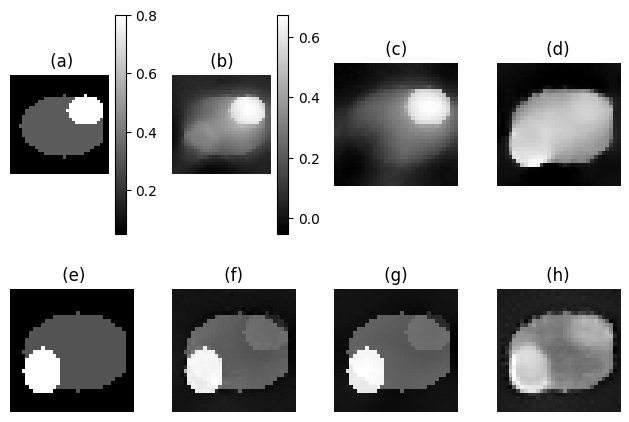
\includegraphics[width=0.7\linewidth]{files/08d41d6e49c649d7c6a2b58601272b38.png}

\begin{verbatim}
import matplotlib.pyplot as plt
import matplotlib.gridspec as gridspec

fig = plt.figure(figsize=(12, 6))
gs = gridspec.GridSpec(2, 5, width_ratios=[1, 1, 1, 1, 0.05], wspace=0.3)

# First row
ax1 = fig.add_subplot(gs[0, 0])
im = ax1.imshow(phantom_water[:, :, objectSize//2], cmap='gray')
ax1.set_title(' (a)')
ax1.axis('off')

ax2 = fig.add_subplot(gs[0, 1])
ax2.imshow(best_water_image[:, :, objectSize//2], cmap='gray')
ax2.set_title(' (b)')
ax2.axis('off')

ax3 = fig.add_subplot(gs[0, 2])
ax3.imshow(last_water_image[:, :, objectSize//2], cmap='gray')
ax3.set_title(' (c)')
ax3.axis('off')

ax4 = fig.add_subplot(gs[0, 3])
ax4.imshow(model_water[:, :, objectSize//2], cmap='gray')
ax4.set_title(' (d)')
ax4.axis('off')

# Second row
ax5 = fig.add_subplot(gs[1, 0])
ax5.imshow(phantom_bone[:, :, objectSize//2], cmap='gray')
ax5.set_title(' (e)')
ax5.axis('off')

ax6 = fig.add_subplot(gs[1, 1])
ax6.imshow(best_bone_image[:, :, objectSize//2], cmap='gray')
ax6.set_title(' (f)')
ax6.axis('off')

ax7 = fig.add_subplot(gs[1, 2])
ax7.imshow(last_bone_image[:, :, objectSize//2], cmap='gray')
ax7.set_title(' (g)')
ax7.axis('off')

ax8 = fig.add_subplot(gs[1, 3])
ax8.imshow(model_bone[:, :, objectSize//2], cmap='gray')
ax8.set_title(' (h)')
ax8.axis('off')

# Add colorbar on dedicated axis (right column)
cax = fig.add_subplot(gs[:, 4])
fig.colorbar(im, cax=cax)

# fig.tight_layout()
plt.show()
\end{verbatim}

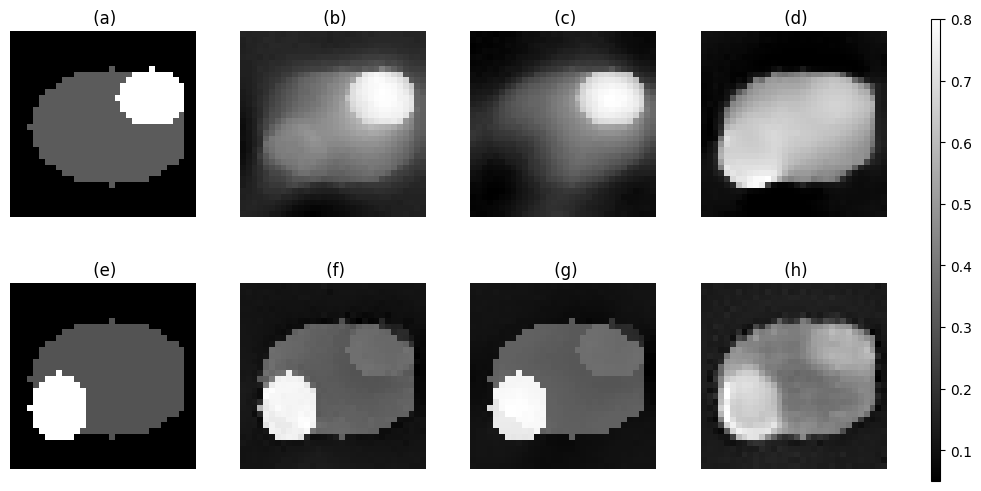
\includegraphics[width=0.7\linewidth]{files/bdda59cec4f2e4c72b6b8b7af0f49ee7.png}